%
%  untitled
%
%  Created by andrea crotti on 2009-03-09.
%  Copyright (c) 2009 Andrea Crotti Corp. All rights reserved.
%
\documentclass[]{article}

% Use utf-8 encoding for foreign characters
\usepackage[utf8]{inputenc}

% Setup for fullpage use
\usepackage{fullpage}

% Uncomment some of the following if you use the features
%
% Running Headers and footers
%\usepackage{fancyhdr}

% Multipart figures
%\usepackage{subfigure}

% More symbols
%\usepackage{amsmath}
%\usepackage{amssymb}
%\usepackage{latexsym}

% Surround parts of graphics with box
\usepackage{boxedminipage}

% Package for including code in the document
\usepackage{listings}

% If you want to generate a toc for each chapter (use with book)
\usepackage{minitoc}

% This is now the recommended way for checking for PDFLaTeX:
\usepackage{ifpdf}

\ifpdf
\usepackage[pdftex]{graphicx}
\else
\usepackage{graphicx}
\fi
\title{Nomadic communication relation}
\author{Andrea Crotti, Fabio Cannioto, Alberto Scattolo, Christian Plattner}

\date{2009-03-09}

\begin{document}

\ifpdf
\DeclareGraphicsExtensions{.pdf, .jpg, .tif}
\else
\DeclareGraphicsExtensions{.eps, .jpg}
\fi

\maketitle
\lstset{numbers=left, numberstyle=\tiny, language=python}

\section{Intro}
% Describe what we are gonna do, the general ideas and what we are gonna talk about.
% Say what is needed to understand the sections that will follow.

The purpose of the project 
is the evaluation of the performances variation of a wireless network 802.11 b/g at the change of some parameters.
\\\newline
In order to make those tests we used some tools whitch are Iperf, wireshark, and a complex python script for the automated run test.
\\\newline
The test consist basicaly in many automatic execution of iperf with fixed time and different speed and finaly we consider the amount of transfering data.
\\\newline
The set of the tests was an indoor environment a notebook wich run iperf as server, an other notebook wich run iperf as client (throw the python script), a cisco ap and another notebook wich run wireshark to sniff the traffic.

\vspace{1cm}

\begin{figure}[h!]
	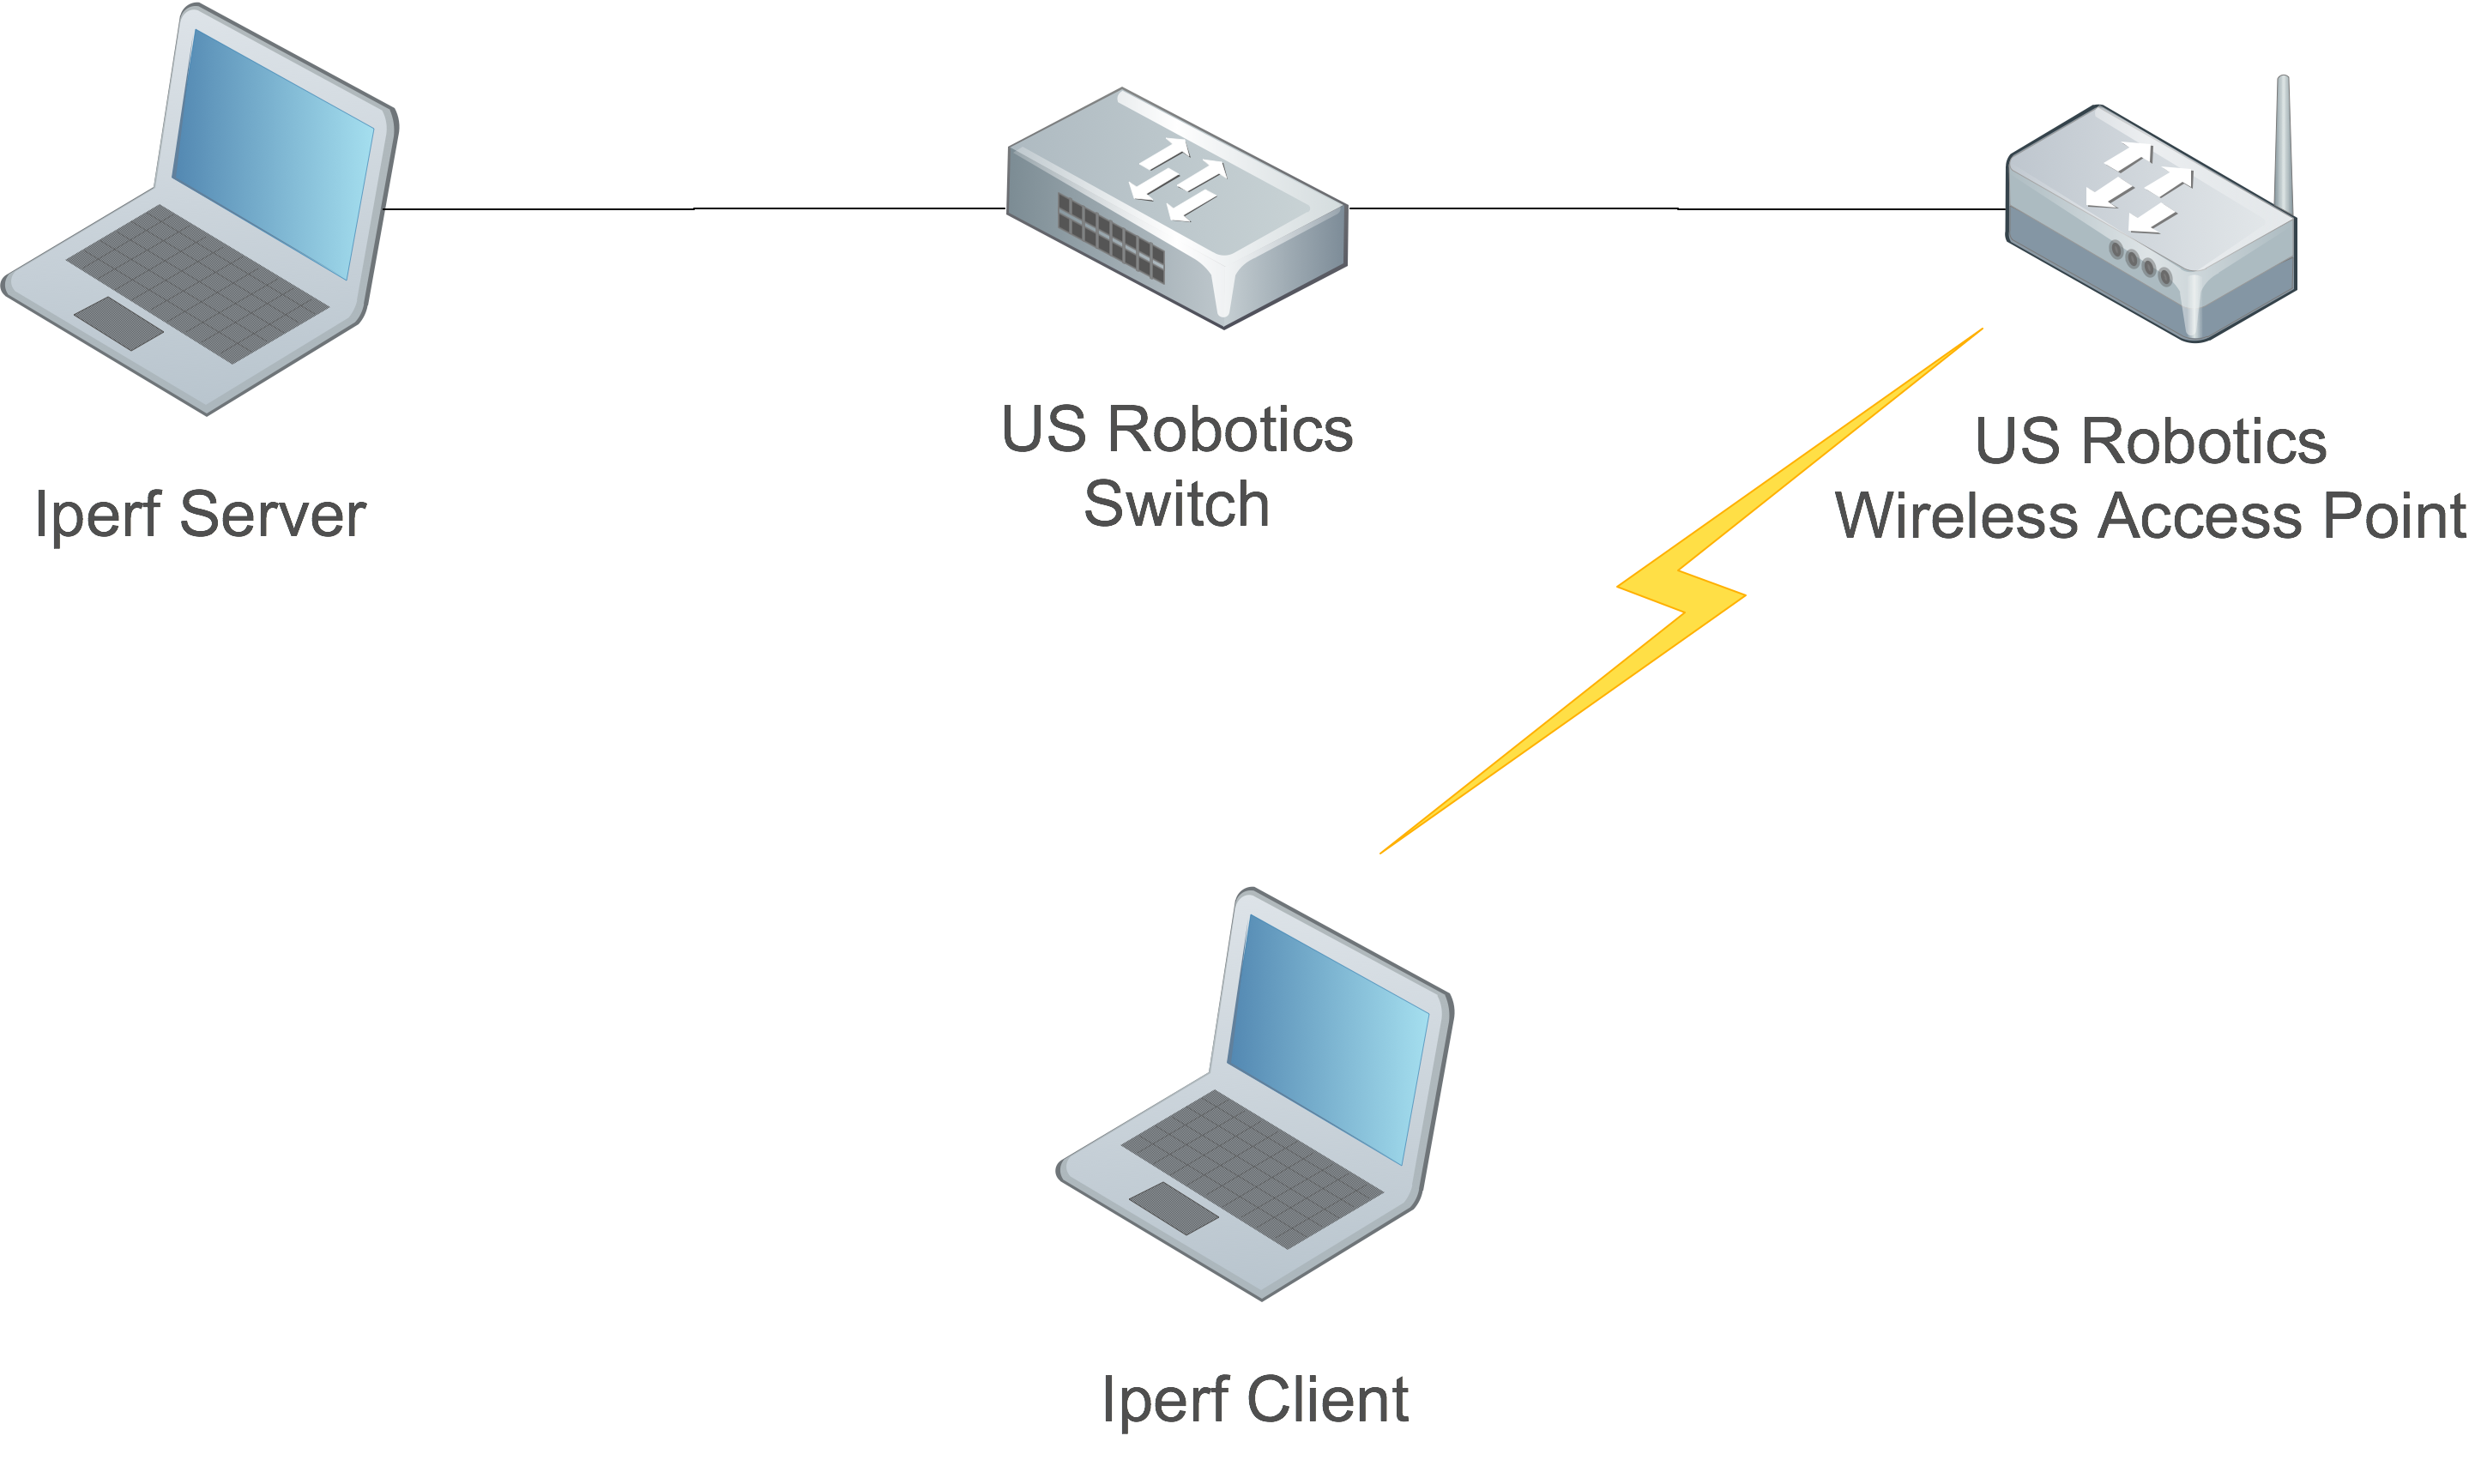
\includegraphics[angle=0, keepaspectratio=true, width=15cm]{images/network_overview}
	\caption{Network overview}
\end{figure}


\section{Theoretical background}
% Everything that comes from theory and that is needed to understand and describe our work.
	\subsection{802.11} \label{theory:prot_specs}
	802.11 is the standard family of protocols for wireless networks. It is also named Wi-Fi. 802.11 protocols family describe how various wireless devices must interact. Nowadays the most popular 802.11 implementation are 802.11b and 802.11g.
	
% A simple description of how an IEEE 802.11 protocol works to introduce the fact that there is some overhead added by the protocol.
% Yes, I know it's unbelivable but there are some differences, for real! :)
	\subsection{Differences between 802.11b and 802.11g} \label{theory:prot_differences}
	
	802.11b protocol was born in October 1999 and since this date it has a discrete success but with the advent of some other wireless device such as cordless telephones it suffer interfernce that causes slower performance. 802.11b extends the basic net bit rate of the standard 802.11 up to 11 Mbit/s.\\
	
	In June 2003 arrives 802.11g that is fully backwards compatible with 802.11b but has best bit rates and throughput\\
	Both protocols use the same frequency band (2.4 GHz) but use different frequency spreads. While 802.11b use direct sequence spread spectrum signaling (DSSS), 802.11g use orthogonal frequency division multiplexing (OFDM) methods. Because of OFDM 802.11g increase the net bit rate up tu 54 Mbit/s.
	
	\begin{table}[h]
		
		\begin{tabularx}{15cm}{ | X X X X X X | }
			\hline
				802.11 Protocol & Release & Freq. (GHz) & Typ throughput (Mbit/s) & Max net bitrate (Mbit/s) & Modulation \\
			\hline
				-- & Jun 1997 & 2.4 & 00.9 & 002 & DSSS \\
				b & Sep 1999 & 2.4 & 04.3 & 011 & DSSS \\
				g & Jun 2003 & 2.4 & 19 & 054 & OFDM \\
			\hline
		\end{tabularx}
		
		\caption{802.11 family standard}
		\label{802.11_family_standard}
	\end{table}
	
	As we can see from the table the standard g's typical throughput is just shy of fivefold then b standard typical throughput and the main difference is the modulation method.

		% Calculate protocols upperbound limitations and similar things (report the formulas!).
		% DO NOT USE PROFESSOR SLIDES AS SOURCE OF INFORMATIONS SINCE MOST OF VALUES ARE COMPLETELY WRONG!!!!!!!!!
		% Download the IEEE standard from here: http://disi.unitn.it/locigno/didattica/NC/802.11-2007.pdf and make a large use of ^F.


\section{Software setup}
\subsection{Software} \label{setup:software}
	% ssh keys, iwconfig, python software, iperf, tcpdump, gnuplot, whatever used


\section{Hardware setup}
\subsection{Hardware} \label{setup:hardware}
	% mainly C wifi card configuration, ap settings

\noindent
For the experiment we were provided with some devices by the university, however, we decided to use our own equipment for doing the tests.

Our iperf server and client were run on different notebooks, as shown in table \ref{tbl:laptops}. Furthermore, the network consists of an US Robotics Access Point and a switch from the same company (table \ref{tbl:networkdevices}).


%\subsubsection{Laptops}
%	\begin{tabular*}{1\textwidth}{@{\extracolsep{\fill}} | l l | }
	\begin{table}[h]
		
		\begin{tabularx}{15cm}{ | m{4cm} X | }
			\hline
				ROLE & Client\\
				MODEL & HP Pavilion dv5-1070el\\
				WIFI & Intel PRO/Wireless 5100 AGN\\
				FIRMWERE & iwlwifi-5000 - 6 October 2008\\
			\hline
		\end{tabularx}
		\\\\\\
		\begin{tabularx}{15cm}{ | m{4cm} X | }
			\hline
				ROLE & Server\\
				MODEL & Asus M2410L\\
				WIFI & Intel PRO/Wireless LAN 2100 3B Mini PCI\\
				FIRMWERE & ipw2100\\
			\hline
		\end{tabularx}
		
		\caption{Laptop configuration}
		\label{table1}
		\label{tbl:laptops}
	\end{table}

%\subsubsection{Network devices}
	\begin{table}[h]
		
		\begin{tabularx}{15cm}{ | m{4cm} X | }
			\hline
				ROLE & Access Point\\
				MODEL & US Robotics 805450\\
				FIRMWERE & version 1.53\\
			\hline
		\end{tabularx}
		\\\\\\
		\begin{tabularx}{15cm}{ | m{4cm} X | }
			\hline
				ROLE & Switch\\
				MODEL & US Robotics\\
			\hline
		\end{tabularx}
		
		\caption{Network devices configuration}
		\label{table2}
		\label{tbl:networkdevices}
	\end{table}


\section{Results analysis}
The tests we executed are in order
%(andrea/tests)s

\begin{figure}
    
\end{figure}

\bibliographystyle{plain}
\bibliography{}
\end{document}
